\documentclass[fleqn]{article}
\usepackage[a4paper, left=1.5cm, right=1.5cm, top=1.5cm, bottom=1.5cm]{geometry}
\usepackage{amsmath}
\usepackage{helvet}
\usepackage{tikz}
\usepackage{bm}

\renewcommand{\familydefault}{\sfdefault}
\DeclareMathOperator*{\argmax}{arg\,max}
\usetikzlibrary{positioning}

\begin{document}

\section*{Setup Context BFE (current timestep $t=1$)}

\begin{figure}[htbp]
    \centering

    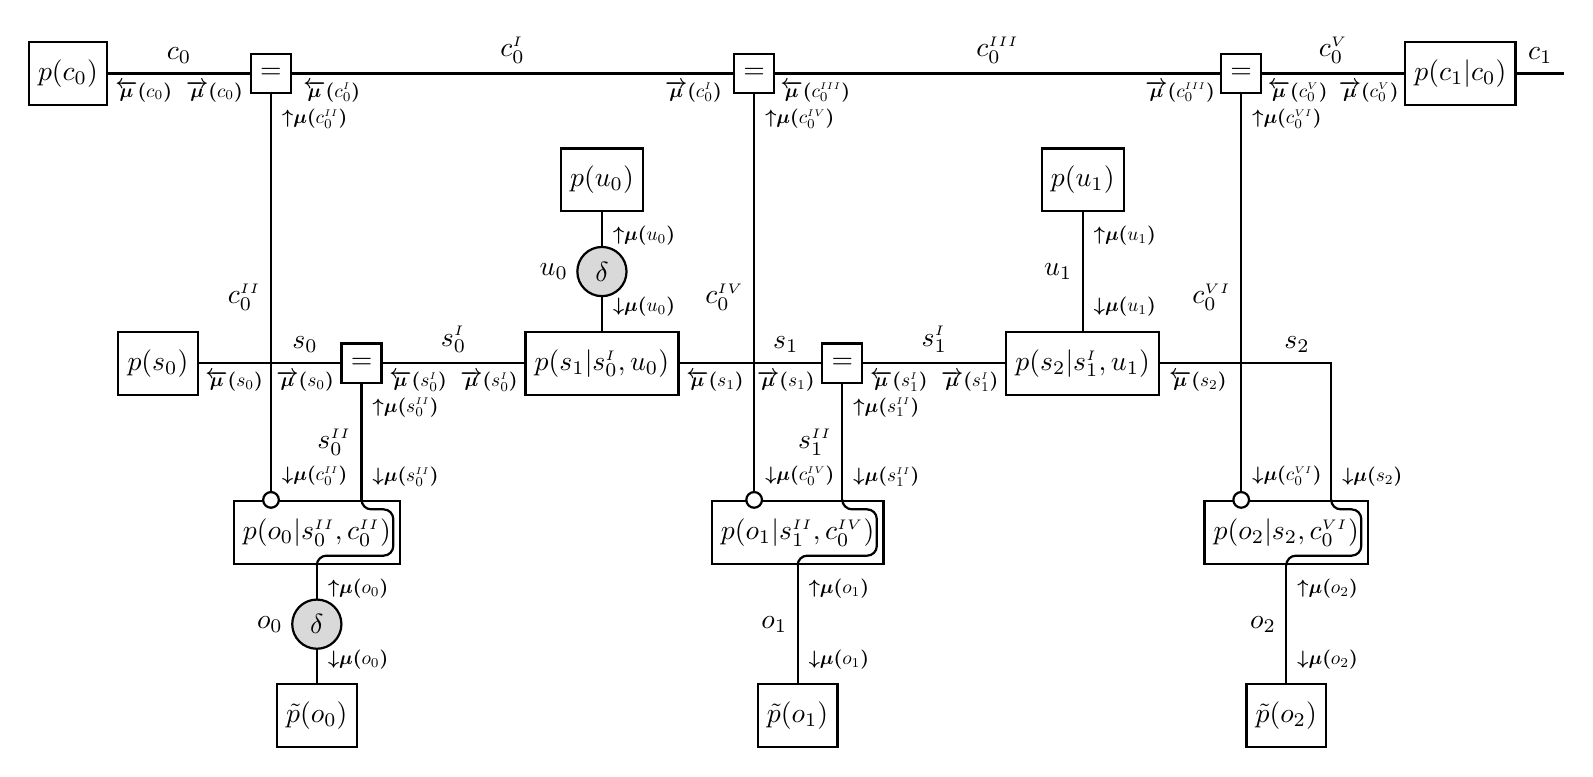
\begin{tikzpicture}[
            factor/.style={draw=black, thick, rectangle, minimum size=0.8cm, font=\normalsize},
            eqfactor/.style={draw=black, thick, rectangle, minimum size=0.5cm, font=\normalsize},
            edge/.style={thick},
            varlabel/.style={font=\normalsize},
            greycircle/.style={draw=black, thick, circle, fill=gray!30, minimum size=0.5cm, font=\normalsize}
        ]

        % Knoten
        \node[factor] (d) {$p(s_0)$};
        \node[eqfactor, right=1.8cm of d] (eq0) {$=$};
        \node[factor] (A0) at ([xshift=1.5cm, yshift=-2.15cm] d.east) {$p(o_0|s^{\scriptscriptstyle II}_0,c^{\scriptscriptstyle II}_0)$};
        \node[factor, below=1.5cm of A0] (c0) {$\tilde{p}(o_0)$};
        \node[factor, right=1.8cm of eq0] (B0) {$p(s_1|s^{\scriptscriptstyle I}_0,u_0)$};
        \node[eqfactor, right=1.8cm of B0] (eq1) {$=$};
        \node[factor] (A1) at ([xshift=1.5cm, yshift=-2.15cm] B0.east) {$p(o_1|s^{\scriptscriptstyle II}_1,c^{\scriptscriptstyle IV}_0)$};
        \node[factor, below=1.5cm of A1] (c1) {$\tilde{p}(o_1)$};
        \node[factor, right=1.8cm of eq1] (B1) {$p(s_2|s^{\scriptscriptstyle I}_1,u_1)$};
        \node[factor] (A2) at ([xshift=1.6cm] B1.east |- A1) {$p(o_2|s_2,c^{\scriptscriptstyle VI}_0)$};
        \node[factor, below=1.5cm of A2] (c2) {$\tilde{p}(o_2)$};
        \node[factor, above=1.5cm of B0] (u0) {$p(u_0)$};
        \node[factor, above=1.5cm of B1] (u1) {$p(u_1)$};
        \node[eqfactor, above right=3cm and 0.65cm of d] (eq3) {$=$};
        \node[eqfactor, right=5.6cm of eq3] (eq4) {$=$};
        \node[eqfactor, right=5.65cm of eq4] (eq5) {$=$};
        \node[factor, left=1.8cm of eq3] (dc) {$p(c_0)$};
        \node[factor, right=1.8cm of eq5] (Bc) {$p(c_1|c_0)$};

        % Kanten zwischen Knoten
        \draw[edge] (d.east) -- (eq0.west) node[pos=0.75, above, varlabel] {$s_0$} node[near start, below, varlabel, scale=0.7] {$\bm{\overleftarrow{\mu}(}s_0\bm{)}$} node[near end, below, varlabel, scale=0.7] {$\bm{\overrightarrow{\mu}(}s_0\bm{)}$};

        \draw[edge] (eq0.south) -- (eq0.south |- A0.north) node[midway, left, varlabel] {$s^{\scriptscriptstyle II}_0$} node[pos=0.2, right=0.05, varlabel, scale=0.7] {$\bm{{\uparrow}{\mu}(}s^{\scriptscriptstyle II}_0\bm{)}$} node[pos=0.8, right=0.05, varlabel, scale=0.7] {$\bm{{\downarrow}{\mu}(}s^{\scriptscriptstyle II}_0\bm{)}$} {};

        \draw[edge] (A0.south) -- (c0.north) node[midway, greycircle] {$\delta$} node[midway, left=0.3cm, varlabel] {$o_0$} node[pos=0.2, right=0.05, varlabel, scale=0.7] {$\bm{{\uparrow}{\mu}(}o_0\bm{)}$} node[pos=0.8, right=0.05, varlabel, scale=0.7] {$\bm{{\downarrow}{\mu}(}o_0\bm{)}$} {};

        \draw[edge] (eq0.east) -- (B0.west) node[midway, above, varlabel] {$s^{\scriptscriptstyle I}_0$} node[near start, below, varlabel, scale=0.7] {$\bm{\overleftarrow{\mu}(}s^{\scriptscriptstyle I}_0\bm{)}$} node[near end, below, varlabel, scale=0.7] {$\bm{\overrightarrow{\mu}(}s^{\scriptscriptstyle I}_0\bm{)}$};

        \draw[edge] (B0.north) -- (u0.south) node[midway, greycircle] {$\delta$} node[midway, left=0.3, varlabel] {$u_0$} node[pos=0.8, right=0.05, varlabel, scale=0.7] {$\bm{{\uparrow}{\mu}(}u_0\bm{)}$} node[pos=0.2, right=0.05, varlabel, scale=0.7] {$\bm{{\downarrow}{\mu}(}u_0\bm{)}$};

        \draw[edge] (B0.east) -- (eq1.west) node[pos=0.75, above, varlabel] {$s_1$} node[near start, below, varlabel, scale=0.7] {$\bm{\overleftarrow{\mu}(}s_1\bm{)}$} node[near end, below, varlabel, scale=0.7] {$\bm{\overrightarrow{\mu}(}s_1\bm{)}$};

        \draw[edge] (eq1.south) -- (eq1.south |- A1.north) node[midway, left, varlabel] {$s^{\scriptscriptstyle II}_1$} node[pos=0.2, right=0.05, varlabel, scale=0.7] {$\bm{{\uparrow}{\mu}(}s^{\scriptscriptstyle II}_1\bm{)}$} node[pos=0.8, right=0.05, varlabel, scale=0.7] {$\bm{{\downarrow}{\mu}(}s^{\scriptscriptstyle II}_1\bm{)}$} {};

        \draw[edge] (A1.south) -- (c1.north) node[midway, left, varlabel] {$o_1$} node[pos=0.2, right=0.05, varlabel, scale=0.7] {$\bm{{\uparrow}{\mu}(}o_1\bm{)}$} node[pos=0.8, right=0.05, varlabel, scale=0.7] {$\bm{{\downarrow}{\mu}(}o_1\bm{)}$} {};

        \draw[edge] (eq1.east) -- (B1.west) node[midway, above, varlabel] {$s^{\scriptscriptstyle I}_1$} node[near start, below, varlabel, scale=0.7] {$\bm{\overleftarrow{\mu}(}s^{\scriptscriptstyle I}_1\bm{)}$} node[near end, below, varlabel, scale=0.7] {$\bm{\overrightarrow{\mu}(}s^{\scriptscriptstyle I}_1\bm{)}$};

        \draw[edge] (B1.east) -| ([xshift=0.57cm]A2.north) node[pos=0.4, above, varlabel] {$s_2$} node[pos=0.11, below, varlabel, scale=0.7] {$\bm{\overleftarrow{\mu}(}s_2\bm{)}$} node[pos=0.915, right=0.05, varlabel, scale=0.7] {$\bm{{\downarrow}{\mu}(}s_2\bm{)}$} {};

        \draw[edge] (A2.south) -- (c2.north) node[midway, left, varlabel] {$o_2$} node[pos=0.2, right=0.05, varlabel, scale=0.7] {$\bm{{\uparrow}{\mu}(}o_2\bm{)}$} node[pos=0.8, right=0.05, varlabel, scale=0.7] {$\bm{{\downarrow}{\mu}(}o_2\bm{)}$} {};

        \draw[edge] (B1.north) -- (u1.south) node[midway, left, varlabel] {$u_1$} node[pos=0.8, right=0.05, varlabel, scale=0.7] {$\bm{{\uparrow}{\mu}(}u_1\bm{)}$} node[pos=0.2, right=0.05, varlabel, scale=0.7] {$\bm{{\downarrow}{\mu}(}u_1\bm{)}$};

        \draw[edge] (dc.east) -- (eq3.west) node[midway, above, varlabel] {$c_0$} node[near start, below, varlabel, scale=0.7] {$\bm{\overleftarrow{\mu}(}c_0\bm{)}$} node[near end, below, varlabel, scale=0.7] {$\bm{\overrightarrow{\mu}(}c_0\bm{)}$};

        \draw[edge] (eq3.east) -- (eq4.west) node[midway, above, varlabel] {$c^{\scriptscriptstyle I}_0$} node[pos=0.09, below, varlabel, scale=0.7] {$\bm{\overleftarrow{\mu}(}c^{\scriptscriptstyle I}_0\bm{)}$} node[pos=0.91, below, varlabel, scale=0.7] {$\bm{\overrightarrow{\mu}(}c^{\scriptscriptstyle I}_0\bm{)}$};

        \draw[edge] (eq4.east) -- (eq5.west) node[midway, above, varlabel] {$c^{\scriptscriptstyle III}_0$} node[pos=0.09, below, varlabel, scale=0.7] {$\bm{\overleftarrow{\mu}(}c^{\scriptscriptstyle III}_0\bm{)}$} node[pos=0.91, below, varlabel, scale=0.7] {$\bm{\overrightarrow{\mu}(}c^{\scriptscriptstyle III}_0\bm{)}$};

        \draw[edge] (eq5.east) -- (Bc.west) node[midway, above, varlabel] {$c^{\scriptscriptstyle V}_0$} node[near start, below, varlabel, scale=0.7] {$\bm{\overleftarrow{\mu}(}c^{\scriptscriptstyle V}_0\bm{)}$} node[near end, below, varlabel, scale=0.7] {$\bm{\overrightarrow{\mu}(}c^{\scriptscriptstyle V}_0\bm{)}$};

        \draw[edge] (eq3.south) -- (eq3.south |- A0.north) node[midway, left, varlabel] {$c^{\scriptscriptstyle II}_0$} node[pos=0.06, right=0.05, varlabel, scale=0.7] {$\bm{{\uparrow}{\mu}(}c^{\scriptscriptstyle II}_0\bm{)}$} node[pos=0.94, right=0.05, varlabel, scale=0.7] {$\bm{{\downarrow}{\mu}(}c^{\scriptscriptstyle II}_0\bm{)}$} node[pos=1, circle, draw=black, fill=white, inner sep=2pt] {};

        \draw[edge] (eq4.south) -- (eq4.south |- A1.north) node[midway, left, varlabel] {$c^{\scriptscriptstyle IV}_0$} node[pos=0.06, right=0.05, varlabel, scale=0.7] {$\bm{{\uparrow}{\mu}(}c^{\scriptscriptstyle IV}_0\bm{)}$} node[pos=0.94, right=0.05, varlabel, scale=0.7] {$\bm{{\downarrow}{\mu}(}c^{\scriptscriptstyle IV}_0\bm{)}$} node[pos=1, circle, draw=black, fill=white, inner sep=2pt] {};

        \draw[edge] (eq5.south) -- (eq5.south |- A2.north) node[midway, left, varlabel] {$c^{\scriptscriptstyle VI}_0$} node[pos=0.06, right=0.05, varlabel, scale=0.7] {$\bm{{\uparrow}{\mu}(}c^{\scriptscriptstyle VI}_0\bm{)}$} node[pos=0.94, right=0.05, varlabel, scale=0.7] {$\bm{{\downarrow}{\mu}(}c^{\scriptscriptstyle VI}_0\bm{)}$} node[pos=1, circle, draw=black, fill=white, inner sep=2pt] {};

        \draw[edge] (Bc.east) -- ++(0.6cm, 0) node[midway, above, varlabel] {$c_1$};

        \draw[edge, rounded corners=3.5pt]
        (eq0.south |- A0.north)
        -- ([yshift=-0.12cm]eq0.south |- A0.north)
        -| ([xshift=-0.1cm]A0.east)
        |- ([yshift=0.12cm]A0.south)
        -- (A0.south);

        \draw[edge, rounded corners=3.5pt]
        (eq1.south |- A1.north)
        -- ([yshift=-0.12cm]eq1.south |- A1.north)
        -| ([xshift=-0.1cm]A1.east)
        |- ([yshift=0.12cm]A1.south)
        -- (A1.south);

        \draw[edge, rounded corners=3.5pt]
        ([xshift=0.57cm]A2.north)
            -- ([xshift=0.57cm, yshift=-0.12cm]A2.north)
        -| ([xshift=-0.1cm]A2.east)
        |- ([yshift=0.12cm]A2.south)
        -- (A2.south);

    \end{tikzpicture}

    %\caption{CFFG}
    \label{fig:3}
\end{figure}

\noindent
\setlength{\jot}{0.3em}
\begin{minipage}[t]{0.5\textwidth}
    \begin{alignat}{2}
         & \rlap{\text{\bfseries Bethe Forward Sweep (s, u and o):}} \nonumber                                                                                                                                                                                    \\
         & \bm{\overrightarrow{\mu}(}s_0\bm{)}                                  &  & = p(s_0)                                                                                                                                                                     \\
         & \bm{{\uparrow}{\mu}(}o_0\bm{)}                                       &  & = \delta_{o_0, \hat{o_0}}                                                                                                                                                    \\
         & \tilde{f}(o_0,s^{\scriptscriptstyle II}_0)                           &  & = \exp \biggl(\sum_{c^{\scriptscriptstyle II}_0} q(c^{\scriptscriptstyle II}_0) \log p(o_0|s^{\scriptscriptstyle II}_0,c^{\scriptscriptstyle II}_0) \biggr)                  \\
         & \bm{{\uparrow}{\mu}(}s^{\scriptscriptstyle II}_0\bm{)}               &  & = \sum_{o_0} \tilde{f}(o_0,s^{\scriptscriptstyle II}_0) \bm{{\uparrow}{\mu}(}o_0\bm{)}                                                                                       \\
         & \bm{\overrightarrow{\mu}(}s^{\scriptscriptstyle I}_0\bm{)}           &  & = \bm{\overrightarrow{\mu}(}s_0\bm{)} \bm{{\uparrow}{\mu}(}s^{\scriptscriptstyle II}_0\bm{)}                                                                                 \\
         & \bm{{\downarrow}{\mu}(}u_0\bm{)}                                     &  & = \delta_{u_0,\hat{u}_o}                                                                                                                                                     \\
         & \bm{\overrightarrow{\mu}(}s_1\bm{)}                                  &  & = \sum_{s^{\scriptscriptstyle I}_0, u_0} \bm{\overrightarrow{\mu}(}s^{\scriptscriptstyle I}_0\bm{)} \bm{{\downarrow}{\mu}(}u_0\bm{)} p(s_1|{s^{\scriptscriptstyle I}_0},u_0) \\
         & \bm{{\uparrow}{\mu}(}o_1\bm{)}                                       &  & = \tilde{p}(o_1)                                                                                                                                                             \\
         & \tilde{f}(o_1,s^{\scriptscriptstyle II}_1)                           &  & = \exp \biggl(\sum_{c^{\scriptscriptstyle IV}_0} q(c^{\scriptscriptstyle IV}_0) \log p(o_1|s^{\scriptscriptstyle II}_1,c^{\scriptscriptstyle IV}_0) \biggr)                  \\
         & \bm{{\uparrow}{\mu}(}s^{\scriptscriptstyle II}_1\bm{)}               &  & = \sum_{o_1} \tilde{f}(o_1,s^{\scriptscriptstyle II}_1) \bm{{\uparrow}{\mu}(}o_1\bm{)}                                                                                       \\
         & \bm{\overrightarrow{\mu}(}s^{\scriptscriptstyle I}_1\bm{)}           &  & = \bm{\overrightarrow{\mu}(}s_1\bm{)} \bm{{\uparrow}{\mu}(}s^{\scriptscriptstyle II}_1\bm{)}                                                                                 \\
         & \bm{{\downarrow}{\mu}(}u_1\bm{)}                                     &  & = p(u_1)                                                                                                                                                                     \\
         & \bm{{\downarrow}{\mu}(}s_2\bm{)}                                     &  & = \sum_{s^{\scriptscriptstyle I}_1, u_1} \bm{\overrightarrow{\mu}(}s^{\scriptscriptstyle I}_1\bm{)} \bm{{\downarrow}{\mu}(}u_1\bm{)} p(s_2|{s^{\scriptscriptstyle I}_1},u_1) \\
         & \tilde{f}(o_2,s_2)                                                   &  & = \exp \biggl(\sum_{c^{\scriptscriptstyle VI}_0} q(c^{\scriptscriptstyle VI}_0) \log p(o_2|s_2,c^{\scriptscriptstyle VI}_0) \biggr)                                          \\
         & \bm{{\downarrow}{\mu}(}o_2\bm{)}                                     &  & = \sum_{s_2} \tilde{f}(o_2,s_2) \bm{{\downarrow}{\mu}(}s_2\bm{)}                                                                                                             \\
         & \rlap{\text{\bfseries Bethe Backward Sweep (s, u and o):}} \nonumber                                                                                                                                                                                   \\
         & \bm{{\uparrow}{\mu}(}o_2\bm{)}                                       &  & = \tilde{p}(o_2)                                                                                                                                                             \\
         & \bm{\overleftarrow{\mu}(}s_2\bm{)}                                   &  & = \sum_{o_2} \tilde{f}(o_2,s_2) \bm{{\uparrow}{\mu}(}o_2\bm{)}
    \end{alignat}
\end{minipage}%
\begin{minipage}[t]{0.5\textwidth}
    \begin{alignat}{2}
         & \bm{{\uparrow}{\mu}(}u_1\bm{)}                                   &  & = \sum_{s^{\scriptscriptstyle I}_1, s_2} \bm{\overrightarrow{\mu}(}s^{\scriptscriptstyle I}_1\bm{)} \bm{\overleftarrow{\mu}(}s_2\bm{)} p(s_2|{s^{\scriptscriptstyle I}_1},u_1) \\
         & \bm{\overleftarrow{\mu}(}s^{\scriptscriptstyle I}_1\bm{)}        &  & = \sum_{u_1, s_2} \bm{{\downarrow}{\mu}(}u_1\bm{)} \bm{\overleftarrow{\mu}(}s_2\bm{)} p(s_2|s^{\scriptscriptstyle I}_1,u_1)                                                    \\
         & \bm{{\downarrow}{\mu}(}s^{\scriptscriptstyle II}_1\bm{)}         &  & = \bm{\overrightarrow{\mu}(}s_1\bm{)} \bm{\overleftarrow{\mu}(}s^{\scriptscriptstyle I}_1\bm{)}                                                                                \\
         & \bm{{\downarrow}{\mu}(}o_1\bm{)}                                 &  & = \sum_{s^{\scriptscriptstyle II}_1} \tilde{f}(o_1,s^{\scriptscriptstyle II}_1) \bm{{\downarrow}{\mu}(}s^{\scriptscriptstyle II}_1\bm{)}                                       \\
         & \bm{\overleftarrow{\mu}(}s_1\bm{)}                               &  & = \bm{{\uparrow}{\mu}(}s^{\scriptscriptstyle II}_1\bm{)} \bm{\overleftarrow{\mu}(}s^{\scriptscriptstyle I}_1\bm{)}                                                             \\
         & \bm{{\uparrow}{\mu}(}u_0\bm{)}                                   &  & = \delta_{u_0, \hat{u}_o}                                                                                                                                                      \\
         & \bm{\overleftarrow{\mu}(}s^{\scriptscriptstyle I}_0\bm{)}        &  & = \sum_{u_o, s_1} \bm{{\downarrow}{\mu}(}u_0\bm{)} \bm{\overleftarrow{\mu}(}s_1\bm{)} p(s_1|s^{\scriptscriptstyle I}_0,u_0)                                                    \\
         & \bm{{\downarrow}{\mu}(}s^{\scriptscriptstyle II}_0\bm{)}         &  & = \bm{\overrightarrow{\mu}(}s_0\bm{)} \bm{\overleftarrow{\mu}(}s^{\scriptscriptstyle I}_0\bm{)}                                                                                \\
         & \bm{{\downarrow}{\mu}(}o_0\bm{)}                                 &  & = \sum_{s^{\scriptscriptstyle II}_0} \tilde{f}(o_0,s^{\scriptscriptstyle II}_0) \bm{{\downarrow}{\mu}(}s^{\scriptscriptstyle II}_0\bm{)}                                       \\
         & \bm{\overleftarrow{\mu}(}s_0\bm{)}                               &  & = \bm{{\uparrow}{\mu}(}s^{\scriptscriptstyle II}_0\bm{)} \bm{\overleftarrow{\mu}(}s^{\scriptscriptstyle I}_0\bm{)}                                                             \\[0.5em]
         & \rlap{\text{\bfseries Updating Beliefs (s, u and o):}} \nonumber                                                                                                                                                                                     \\
         & q(s_0)                                                           &  & \propto \bm{\overleftarrow{\mu}(}s_0\bm{)} \bm{\overrightarrow{\mu}(}s_0\bm{)}                                                                                                 \\
         & q(s^{\scriptscriptstyle I}_0)                                    &  & \propto \bm{\overleftarrow{\mu}(}s^{\scriptscriptstyle I}_0\bm{)} \bm{\overrightarrow{\mu}(}s^{\scriptscriptstyle I}_0\bm{)}                                                   \\
         & q(s^{\scriptscriptstyle II}_0)                                   &  & \propto \bm{{\uparrow}{\mu}(}s^{\scriptscriptstyle II}_0\bm{)} \bm{{\downarrow}{\mu}(}s^{\scriptscriptstyle II}_0\bm{)}                                                        \\
         & q(s_1)                                                           &  & \propto \bm{\overleftarrow{\mu}(}s_1\bm{)} \bm{\overrightarrow{\mu}(}s_1\bm{)}                                                                                                 \\
         & q(s^{\scriptscriptstyle I}_1)                                    &  & \propto \bm{\overleftarrow{\mu}(}s^{\scriptscriptstyle I}_1\bm{)} \bm{\overrightarrow{\mu}(}s^{\scriptscriptstyle I}_1\bm{)}                                                   \\
         & q(s^{\scriptscriptstyle II}_1)                                   &  & \propto \bm{{\uparrow}{\mu}(}s^{\scriptscriptstyle II}_1\bm{)} \bm{{\downarrow}{\mu}(}s^{\scriptscriptstyle II}_1\bm{)}                                                        \\
         & q(s_2)                                                           &  & \propto \bm{\overleftarrow{\mu}(}s_2\bm{)} \bm{{\downarrow}{\mu}(}s_2\bm{)}                                                                                                    \\
         & q(u_0)                                                           &  & \propto \delta_{u_0,\hat{u_0}}                                                                                                                                                 \\
         & q(u_1)                                                           &  & \propto \bm{{\uparrow}{\mu}(}u_1\bm{)} \bm{{\downarrow}{\mu}(}u_1\bm{)}                                                                                                        \\
         & q(o_0)                                                           &  & \propto \delta_{o_0,\hat{o_0}}                                                                                                                                                 \\
         & q(o_1)                                                           &  & \propto \bm{{\uparrow}{\mu}(}o_1\bm{)} \bm{{\downarrow}{\mu}(}o_1\bm{)}                                                                                                        \\
         & q(o_2)                                                           &  & \propto \bm{{\uparrow}{\mu}(}o_1\bm{)} \bm{{\downarrow}{\mu}(}o_2\bm{)}
    \end{alignat}
\end{minipage}

\newpage
\noindent
\setlength{\jot}{0.6em}
\begin{minipage}[t]{0.5\textwidth}
    \begin{alignat}{2}
         & q(o_0,s^{\scriptscriptstyle II}_0)                           &  & \propto \tilde{f}(o_0,s^{\scriptscriptstyle II}_0) \bm{{\downarrow}{\mu}(}s^{\scriptscriptstyle II}_0\bm{)} \bm{{\uparrow}{\mu}(}o_0\bm{)}                           \\
         & q(o_1,s^{\scriptscriptstyle II}_1)                           &  & \propto \tilde{f}(o_1,s^{\scriptscriptstyle II}_1) \bm{{\downarrow}{\mu}(}s^{\scriptscriptstyle II}_1\bm{)} \bm{{\uparrow}{\mu}(}o_1\bm{)}                           \\
         & q(o_2,s_2)                                                   &  & \propto \tilde{f}(o_0,s_2) \bm{{\downarrow}{\mu}(}s_2\bm{)} \bm{{\uparrow}{\mu}(}o_2\bm{)}                                                                           \\
         & \rlap{\text{\bfseries Bethe Forward Sweep (c):}} \nonumber                                                                                                                                                                             \\
         & \bm{\overrightarrow{\mu}(}c_0\bm{)}                          &  & = p(c_0)                                                                                                                                                             \\
         & \bm{{\uparrow}{\mu}(}c^{\scriptscriptstyle II}_0\bm{)}       &  & = \exp \biggl( \sum_{o_0,s^{\scriptscriptstyle II}_0} q(o_0,s^{\scriptscriptstyle II}_0) \log p(o_0|s^{\scriptscriptstyle II}_0,c^{\scriptscriptstyle II}_0) \biggr) \\
         & \bm{\overrightarrow{\mu}(}c^{\scriptscriptstyle I}_0\bm{)}   &  & = \bm{\overrightarrow{\mu}(}c_0\bm{)} \bm{{\uparrow}{\mu}(}c^{\scriptscriptstyle II}_0\bm{)}                                                                         \\
         & \bm{{\uparrow}{\mu}(}c^{\scriptscriptstyle IV}_0\bm{)}       &  & = \exp \biggl( \sum_{o_1,s^{\scriptscriptstyle II}_1} q(o_1,s^{\scriptscriptstyle II}_1) \log p(o_1|s^{\scriptscriptstyle II}_1,c^{\scriptscriptstyle IV}_0) \biggr) \\
         & \bm{\overrightarrow{\mu}(}c^{\scriptscriptstyle III}_0\bm{)} &  & = \bm{\overrightarrow{\mu}(}c^{\scriptscriptstyle I}_0\bm{)} \bm{{\uparrow}{\mu}(}c^{\scriptscriptstyle IV}_0\bm{)}                                                  \\
         & \bm{{\uparrow}{\mu}(}c^{\scriptscriptstyle VI}_0\bm{)}       &  & = \exp \biggl( \sum_{o_2,s_2} q(o_2,s_2) \log p(o_2|s_2,c^{\scriptscriptstyle VI}_0) \biggr)                                                                         \\
         & \bm{\overrightarrow{\mu}(}c^{\scriptscriptstyle V}_0\bm{)}   &  & = \bm{\overrightarrow{\mu}(}c^{\scriptscriptstyle III}_0\bm{)} \bm{{\uparrow}{\mu}(}c^{\scriptscriptstyle VI}_0\bm{)}
    \end{alignat}
\end{minipage}
\begin{minipage}[t]{0.5\textwidth}
    \begin{alignat}{2}
         & \rlap{\text{\bfseries Bethe Backward Sweep (c):}} \nonumber                                                                                                                                               \\
         & \bm{\overleftarrow{\mu}(}c^{\scriptscriptstyle V}_0\bm{)}           &  & = [0.5, 0.5]^T                                                                                                                   \\
         & \bm{{\downarrow}{\mu}(}c^{\scriptscriptstyle VI}_0\bm{)}            &  & = \bm{\overrightarrow{\mu}(}c^{\scriptscriptstyle III}_0\bm{)} \bm{\overleftarrow{\mu}(}c^{\scriptscriptstyle V}_0\bm{)}         \\
         & \bm{\overleftarrow{\mu}(}c^{\scriptscriptstyle III}_0\bm{)}         &  & = \bm{{\uparrow}{\mu}(}c^{\scriptscriptstyle VI}_0\bm{)} \bm{\overleftarrow{\mu}(}c^{\scriptscriptstyle V}_0\bm{)}               \\
         & \bm{{\downarrow}{\mu}(}c^{\scriptscriptstyle IV}_0\bm{)}            &  & = \bm{\overrightarrow{\mu}(}c^{\scriptscriptstyle I}_0\bm{)} \bm{\overleftarrow{\mu}(}c^{\scriptscriptstyle III}_0\bm{)}         \\
         & \bm{\overleftarrow{\mu}(}c^{\scriptscriptstyle I}_0\bm{)}           &  & = \bm{{\uparrow}{\mu}(}c^{\scriptscriptstyle IV}_0\bm{)} \bm{\overleftarrow{\mu}(}c^{\scriptscriptstyle III}_0\bm{)}             \\
         & \bm{{\downarrow}{\mu}(}c^{\scriptscriptstyle II}_0\bm{)}            &  & = \bm{\overrightarrow{\mu}(}c_0\bm{)} \bm{\overleftarrow{\mu}(}c^{\scriptscriptstyle I}_0\bm{)}                                  \\
         & \bm{\overleftarrow{\mu}(}c_0\bm{)}                                  &  & = \bm{{\uparrow}{\mu}(}c^{\scriptscriptstyle II}_0\bm{)} \bm{\overleftarrow{\mu}(}c^{\scriptscriptstyle I}_0\bm{)}               \\
         & \rlap{\text{\bfseries Updating Beliefs (c):}} \nonumber                                                                                                                                                   \\
         & q(c_0)                                                              &  & \propto \bm{\overleftarrow{\mu}(}c_0\bm{)} \bm{\overrightarrow{\mu}(}c_0\bm{)}                                                   \\
         & q(c^{\scriptscriptstyle I}_0)                                       &  & \propto \bm{\overleftarrow{\mu}(}c^{\scriptscriptstyle I}_0\bm{)} \bm{\overrightarrow{\mu}(}c^{\scriptscriptstyle I}_0\bm{)}     \\
         & q(c^{\scriptscriptstyle II}_0)                                      &  & \propto \bm{{\uparrow}{\mu}(}c^{\scriptscriptstyle II}_0\bm{)} \bm{{\downarrow}{\mu}(}c^{\scriptscriptstyle II}_0\bm{)}          \\
         & q(c^{\scriptscriptstyle III}_0)                                     &  & \propto \bm{\overleftarrow{\mu}(}c^{\scriptscriptstyle III}_0\bm{)} \bm{\overrightarrow{\mu}(}c^{\scriptscriptstyle III}_0\bm{)} \\
         & q(c^{\scriptscriptstyle IV}_0)                                      &  & \propto \bm{{\uparrow}{\mu}(}c^{\scriptscriptstyle IV}_0\bm{)} \bm{{\downarrow}{\mu}(}c^{\scriptscriptstyle IV}_0\bm{)}          \\
         & q(c^{\scriptscriptstyle V}_0)                                       &  & \propto \bm{\overleftarrow{\mu}(}c^{\scriptscriptstyle V}_0\bm{)} \bm{\overrightarrow{\mu}(}c^{\scriptscriptstyle V}_0\bm{)}     \\
         & q(c^{\scriptscriptstyle VI}_0)                                      &  & \propto \bm{{\uparrow}{\mu}(}c^{\scriptscriptstyle VI}_0\bm{)} \bm{{\downarrow}{\mu}(}c^{\scriptscriptstyle VI}_0\bm{)}          \\
         & \rlap{\text{\bfseries Repeat Eq.1-63 until convergence!}} \nonumber
    \end{alignat}
\end{minipage}

\begin{alignat*}{2}
    F = & \sum_{s_0} q(s_0) \log \frac{q(s_0)}{p(s_0)} + \sum_{s_1, s^{\scriptscriptstyle I}_0, u_0} q(s_1, s^{\scriptscriptstyle I}_0, u_0) \log \frac{q(s_1, s^{\scriptscriptstyle I}_0, u_0)}{p(s_1| s^{\scriptscriptstyle I}_0, u_0)} + \sum_{s_2, s^{\scriptscriptstyle I}_1, u_1} q(s_2, s^{\scriptscriptstyle I}_1, u_1) \log \frac{q(s_2, s^{\scriptscriptstyle I}_1, u_1)}{p(s_2| s^{\scriptscriptstyle I}_1, u_1)} \\
        & + \sum_{u_0} q(u_0) \log \frac{q(u_0)}{p(u_0)} + \sum_{u_1} q(u_1) \log \frac{q(u_1)}{p(u_1)}                                                                                                                              \\
        & + \sum_{o_0, s^{\scriptscriptstyle II}_0, c^{\scriptscriptstyle II}_0} q(o_0, s^{\scriptscriptstyle II}_0)q(c^{\scriptscriptstyle II}_o) \log \frac{q(o_0, s^{\scriptscriptstyle II}_0)q(c^{\scriptscriptstyle II}_0)}{p(o_0| s^{\scriptscriptstyle II}_0, c^{\scriptscriptstyle II}_0)} + \sum_{o_1, s^{\scriptscriptstyle II}_1, c^{\scriptscriptstyle IV}_0} q(o_1, s^{\scriptscriptstyle II}_1)q(c^{\scriptscriptstyle IV}_0) \log \frac{q(o_1, s^{\scriptscriptstyle II}_1)q(c^{\scriptscriptstyle IV}_0)}{p(o_1| s^{\scriptscriptstyle II}_1, c^{\scriptscriptstyle IV}_0)}                                          \\
        & + \sum_{o_2, s_2, c^{\scriptscriptstyle VI}_0} q(o_2, s_2) q(c^{\scriptscriptstyle VI}_0) \log \frac{q(o_2, s_2)q(c^{\scriptscriptstyle VI}_0)}{p(o_2| s_2, c^{\scriptscriptstyle VI}_0)}                                                                                                                                    \\
        & + \sum_{o_0} q(o_0) \log \frac{q(o_0)}{\tilde{p}(o_0)} + \sum_{o_1} q(o_1) \log \frac{q(o_1)}{\tilde{p}(o_1)} + \sum_{o_2} q(o_2) \log \frac{q(o_2)}{\tilde{p}(o_2)}                                                       \\
        & + \sum_{s_0, s^{\scriptscriptstyle I}_0, s^{\scriptscriptstyle II}_0} q(s_0, s^{\scriptscriptstyle I}_0, s^{\scriptscriptstyle II}_0) \log \frac{q(s_0, s^{\scriptscriptstyle I}_0, s^{\scriptscriptstyle II}_0)}{\delta_{s_0, s^{\scriptscriptstyle I}_0} \delta_{s_0, s^{\scriptscriptstyle II}_0}} + \sum_{s_1, s^{\scriptscriptstyle I}_1, s^{\scriptscriptstyle II}_1} q(s_1, s^{\scriptscriptstyle I}_1, s^{\scriptscriptstyle II}_1) \log \frac{q(s_1, s^{\scriptscriptstyle I}_1, s^{\scriptscriptstyle II}_1)}{\delta_{s_1, s^{\scriptscriptstyle I}_1} \delta_{s_1, s^{\scriptscriptstyle II}_1}} \\
        & + \sum_{c_o} q(c_0) \log \frac{q(c_o)}{p(c_0)}                                                                                                                                                                             \\
        & + \sum_{c_0, c^{\scriptscriptstyle I}_0, c^{\scriptscriptstyle II}_0} q(c_0, c^{\scriptscriptstyle I}_0, c^{\scriptscriptstyle II}_0) \log \frac{q(c_0, c^{\scriptscriptstyle I}_0, c^{\scriptscriptstyle II}_0)}{\delta_{c_0, c^{\scriptscriptstyle I}_0} \delta_{c_0, s^{\scriptscriptstyle II}_0}} + \sum_{c^{\scriptscriptstyle I}_0, c^{\scriptscriptstyle III}_0, c^{\scriptscriptstyle IV}_0} q(c^{\scriptscriptstyle I}_0, c^{\scriptscriptstyle III}_0, c^{\scriptscriptstyle IV}_0) \log \frac{q(c^{\scriptscriptstyle I}_0, c^{\scriptscriptstyle III}_0, c^{\scriptscriptstyle IV}_0)}{\delta_{c^{\scriptscriptstyle I}_0, c^{\scriptscriptstyle III}_0} \delta_{c_0, s^{\scriptscriptstyle IV}_0}} \\
        & + \sum_{c^{\scriptscriptstyle III}_0, c^{\scriptscriptstyle V}_0, c^{\scriptscriptstyle VI}_0} q(c^{\scriptscriptstyle III}_0, c^{\scriptscriptstyle V}_0, c^{\scriptscriptstyle VI}_0) \log \frac{q(c^{\scriptscriptstyle III}_0, c^{\scriptscriptstyle V}_0, c^{\scriptscriptstyle VI}_0)}{\delta_{c^{\scriptscriptstyle III}_0, c^{\scriptscriptstyle V}_0} \delta_{c_0, s^{\scriptscriptstyle VI}_0}} \\
        & - \sum_{s_0} q(s_0) \log q(s_0) - \sum_{s^{\scriptscriptstyle I}_0} q(s^{\scriptscriptstyle I}_0) \log q(s^{\scriptscriptstyle I}_0) - \sum_{s^{\scriptscriptstyle II}_0} q(s^{\scriptscriptstyle II}_0) \log q(s^{\scriptscriptstyle II}_0) \\
        & - \sum_{s_1} q(s_1) \log q(s_1) - \sum_{s^{\scriptscriptstyle I}_1} q(s^{\scriptscriptstyle I}_1) \log q(s^{\scriptscriptstyle I}_1) - \sum_{s^{\scriptscriptstyle II}_1} q(s^{\scriptscriptstyle II}_1) \log q(s^{\scriptscriptstyle II}_1) - \sum_{s_2} q(s_2) \log q(s_2)                                                                                                                          \\
        & - \sum_{u_0} q(u_0) \log q(u_0) - \sum_{u_1} q(u_1) \log q(u_1)                                                                                                                                                            \\
        & - \sum_{o_0} q(o_0) \log q(o_0) - \sum_{o_1} q(o_1) \log q(o_1) - \sum_{o_2} q(o_2) \log q(o_2)                                                                                                                            \\
        & - \sum_{c_0} q(c_0) \log q(c_0) - \sum_{c^{\scriptscriptstyle I}_0} q(c^{\scriptscriptstyle I}_0) \log q(c^{\scriptscriptstyle I}_0) - \sum_{c^{\scriptscriptstyle II}_0} q(c^{\scriptscriptstyle II}_0) \log q(c^{\scriptscriptstyle II}_0) - \sum_{c^{\scriptscriptstyle III}_0} q(c^{\scriptscriptstyle III}_0) \log q(c^{\scriptscriptstyle III}_0) \\
        & - \sum_{c^{\scriptscriptstyle IV}_0} q(c^{\scriptscriptstyle IV}_0) \log q(c^{\scriptscriptstyle IV}_0) - \sum_{c^{\scriptscriptstyle VI}_0} q(c^{\scriptscriptstyle VI}_0) \log q(c^{\scriptscriptstyle VI}_0)
\end{alignat*}

\end{document}
